% -----------------------------------------------------------
% Appendix
% -----------------------------------------------------------

\FloatBarrier
\section{}
\label{appendix}


\begin{figure}
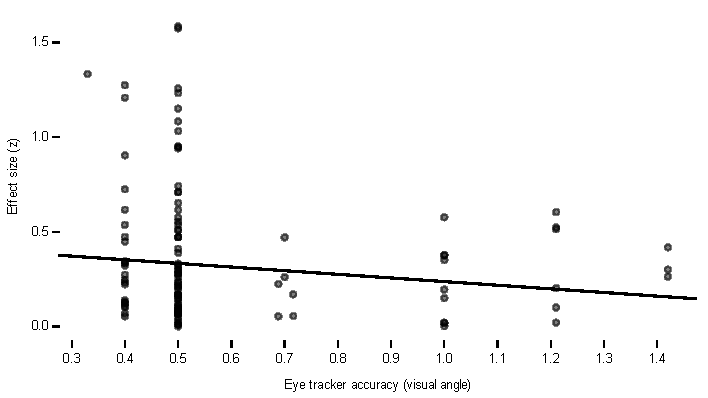
\includegraphics{ET_accuracy_effectsize}
\centering
\caption{\textcolor{Red}{Accuracy of the eye-tracker affects the ability to reliably measure effect sizes in each study. Points denote the accuracy of an eye-tracker used in a study and the effect size measured with it. The line is based on the estimated intercept and slope from the best fitting mixed-effect model which was used to compute artifact multiplier, $a_a$. The multiplier was used to correct for a bias in estimated effect sizes due to differences in measurement accuracy of eye-trackers.}}
\label{fig:ET_accuracy_effectsize}
\end{figure}
\clearpage


% \caption{eye-tracker specifications table}
% \label{tab:eyetracker_specs}
% latex table generated in R 3.5.2 by xtable 1.8-4 package
% Mon Nov 30 09:54:56 2020
\begin{table}[ht]
\centering
\caption{Eye tracker specifications table, with accuracy and precision for each eye tracker as extracted from the manufacturer website, and computed artifact multiplier used for correcting for a bias in effect size estimates.} 
\label{tab:eyetracker_specifications}
\begin{tabular}{lccc}
  \hline
Eye tracker model & $a_a$ & Accuracy & Precision \\ 
  \hline
ASL6000 & 0.5523 & 1.00 & 0.50 \\ 
  Easygaze & 0.6866 & 0.70 & 0.35 \\ 
  Eye gaze 97 & 0.6794 & 0.72 & 0.50 \\ 
  Eye gaze tm & 0.8209 & 0.40 & 0.50 \\ 
  EyeLink 1000 & 0.7762 & 0.50 & 0.05 \\ 
  EyeLink 1000 (acc = .33) & 0.8523 & 0.33 & 0.05 \\ 
  EyeLink 1000 Plus (acc < .5) & 0.7762 & 0.50 & 0.05 \\ 
  EyeLink II & 0.7762 & 0.50 & 0.01 \\ 
  ISCAN & 0.5523 & 1.00 & 0.50 \\ 
  Nihon-Kohden EEG-1100 & 0.5523 & 1.00 & 0.50 \\ 
  SMI Glasses & 0.4583 & 1.21 & 0.19 \\ 
  SMI RED & 0.8209 & 0.40 & 0.03 \\ 
  SMI iview & 0.7762 & 0.50 & 0.01 \\ 
  SMI iview HED & 0.5523 & 1.00 & 0.50 \\ 
  SMI model unknown (acc < .5) & 0.7762 & 0.50 & 0.30 \\ 
  Tobii D10 & 0.7762 & 0.50 & 0.50 \\ 
  Tobii Glasses 1 & 0.3643 & 1.42 & 0.50 \\ 
  Tobii T120 & 0.8209 & 0.40 & 0.24 \\ 
  Tobii T1750 & 0.7762 & 0.50 & 0.25 \\ 
  Tobii T2150 & 0.7762 & 0.50 & 0.35 \\ 
  Tobii T60 & 0.7762 & 0.50 & 0.22 \\ 
  Tobii X1 & 0.7762 & 0.50 & 0.20 \\ 
  Tobii X2 & 0.8209 & 0.40 & 0.32 \\ 
  Tobii X60 & 0.7762 & 0.50 & 0.30 \\ 
  Tobii glasses 2 & 0.3643 & 1.42 & 0.34 \\ 
  Unknown & 0.6919 & 0.69 & 0.30 \\ 
   \hline 
 \multicolumn{4}{l}{\scriptsize{\textit{Note.} $a_a$ = artifact multiplier.}} 
\end{tabular}
\end{table}

\clearpage


\begin{figure}%[H]
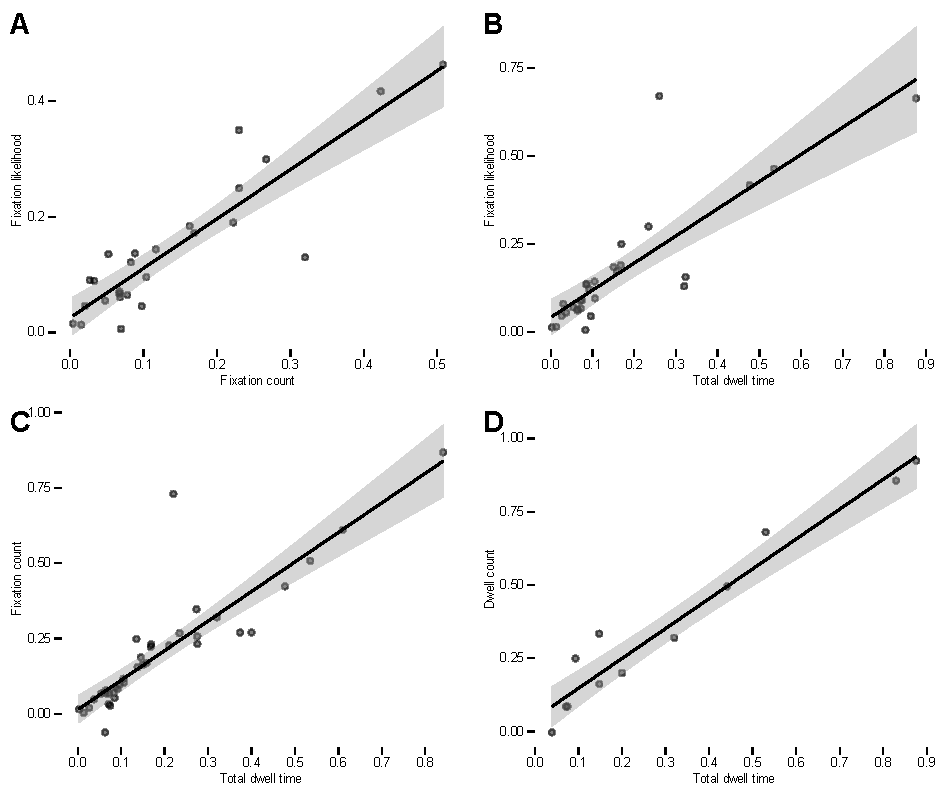
\includegraphics{metric_correction}
\centering
\caption{\textcolor{Red}{Several eye movement metrics are used as dependent variable, but they are all highly correlated, suggesting they are all measuring the same underlying construct. Scatterplots show the relationship (A) between effect sizes expressed in fixation likelihood and fixation count, (B) between total dwell time and fixation likelihood, (C) between total dwell time and fixation count, (D) between total dwell time and dwell count. Lines in each plot represent the best-fitting linear regression line, and the shaded area 95\% confidence interval.}}
\label{fig:metric_correction}
\end{figure}
\clearpage


% \caption{Metric correction factor $a_m$ when correcting to either fixation count or fixation likelihood}
% \label{tab:metric_correction}
% latex table generated in R 3.6.3 by xtable 1.8-4 package
% Fri Dec 18 00:07:07 2020
\begin{table}[ht]
\centering
\caption{Metric correction factor $a_m$ when correcting to either fixation count or fixation likelihood. These correction factors were used to make sure all dependent variables are comparable.} 
\label{tab:metric_correction}
\begin{tabular}{llc}
  \hline
Correcting from & Correcting to & $a_m$ \\ 
  \hline
Fixation count & Fixation likelihood & 1.041 \\ 
  Fixation likelihood & Fixation count & 0.961 \\ 
  Total dwell time & Fixation likelihood & 0.913 \\ 
  Total dwell time & Fixation count & 1.035 \\ 
  Dwell count & Fixation likelihood & 0.844 \\ 
  Dwell count & Fixation count & 0.957 \\ 
   \hline
\end{tabular}
\end{table}

\clearpage


% \caption{Moderator analysis results.}
% \label{tab:mod_results}
% latex table generated in R 3.5.2 by xtable 1.8-4 package
% Mon Apr 19 09:34:50 2021
\begin{table}[ht]
\centering
\caption{Moderator analysis results. The most important values are the corrected effect size estimate, $\rho$, and the associated heterogeneity, $I^2$. 
                Results of the Top10 analysis are in parentheses.} 
\label{tab:mod_results}
\begingroup\small
\begin{tabular}{lccccccccc}
  \hline
Group & $k$ & $N$ & $\rho$ & SE & $Z$ & $p$ & $\textrm{CI}^{95}_{LL}$ & $\textrm{CI}^{95}_{UL}$ & $I^2$ \\ 
  \hline
\textbf{Set size} &  &  &  &  &  &  &  &  &  \\ 
  \hspace{2mm}\textit{Alternative} & 6 & 281 & 0.5 & 0.01 & 48.55 & <0.001 & 0.45 & 0.54 & 0 \\ 
   & (2) & (146) & (0.52) & (0.09) & (6.01) & (<0.001) & (0.35) & (0.69) & (0) \\ 
  \hspace{2mm}\textit{Attribute} & 7 & 726 & 0.14 & 0.05 & 2.88 & 0.035 & 0.02 & 0.27 & 30.38 \\ 
   & (2) & (302) & (0.07) & (0.07) & (0.95) & (0.343) & (-0.07) & (0.21) & (0) \\ 
  \textbf{Task instruction} &  &  &  &  &  &  &  &  &  \\ 
  \hspace{2mm}\textit{Alternative} & 12 & 787 & 0.39 & 0.08 & 4.79 & 0.001 & 0.2 & 0.57 & 10.85 \\ 
   & (2) & (406) & (0.34) & (0.11) & (3.13) & (0.002) & (0.13) & (0.56) & (38.13) \\ 
  \hspace{2mm}\textit{Attribute} & 16 & 1273 & 0.34 & 0.06 & 5.32 & <0.001 & 0.2 & 0.48 & 64.64 \\ 
   & (2) & (468) & (0.28) & (0.1) & (2.67) & (0.008) & (0.07) & (0.48) & (68.33) \\ 
  \textbf{Preferential viewing} &  &  &  &  &  &  &  &  &  \\ 
  \hspace{2mm}\textit{Alternative} & 7 & 600 & 0.61 & 0.19 & 3.17 & 0.034 & 0.08 & 1.13 & 76.81 \\ 
   & (2) & (385) & (0.29) & (0.08) & (3.64) & (<0.001) & (0.13) & (0.45) & (0) \\ 
  \hspace{2mm}\textit{Attribute} & 17 & 2033 & 0.31 & 0.08 & 3.95 & 0.002 & 0.14 & 0.47 & 77.03 \\ 
   & (2) & (688) & (0.31) & (0.13) & (2.43) & (0.015) & (0.06) & (0.55) & (86.6) \\ 
   \hline 
 \multicolumn{10}{p{0.9\textwidth}}{\scriptsize{\textit{Note.} $k$ = number of studies; $N$ = number of participants; $\rho$ = unattenuated effect size estimate, SE = standard error of estimate; $Z$ = Z statistic; $p$ = significance level; $\textrm{CI}^{95}_{LL}$ = lower limit of the 95\% confidence interval; $\textrm{CI}^{95}_{LL}$ = upper limit of the 95\% confidence interval, $I^2$ = within-group heterogeneity.}} 
\end{tabular}
\endgroup
\end{table}

\clearpage


% PET and PEESE result tables
% latex table generated in R 3.5.2 by xtable 1.8-4 package
% Wed Mar 17 09:58:16 2021
\begin{table}[ht]
\centering
\caption{Publication bias analysis with precision-effect test (PET) and precision-effect estimate test (PEESE) of complete data. See \textit{Methods} for details on the tests.} 
\label{tab:PET-PEESE}
\begin{tabular}{lccccc}
  \hline
Parameter & beta & t & $t$ & $p$ & p_Satt \\ 
  \hline
PET &  &  &  &  & PET \\ 
  Intercept & 0.169 & 0.102 & 1.651 & 1.505 & 0.279 \\ 
  $SD$ & 2.156 & 0.622 & 3.468 & 8.888 & 0.007 \\ 
  $A$ & -0.118 & 0.156 & -0.753 & 3.01 & 0.506 \\ 
  PEESE &  &  &  &  & PEESE \\ 
  Intercept & 0.23 & 0.098 & 2.355 & 1.627 & 0.171 \\ 
  $Var$ & 5.598 & 1.886 & 2.969 & 12.94 & 0.011 \\ 
  $A$ & -0.001 & 0.172 & -0.004 & 2.417 & 0.997 \\ 
   \hline
\end{tabular}
\end{table}

\clearpage


\begin{figure}%[H]
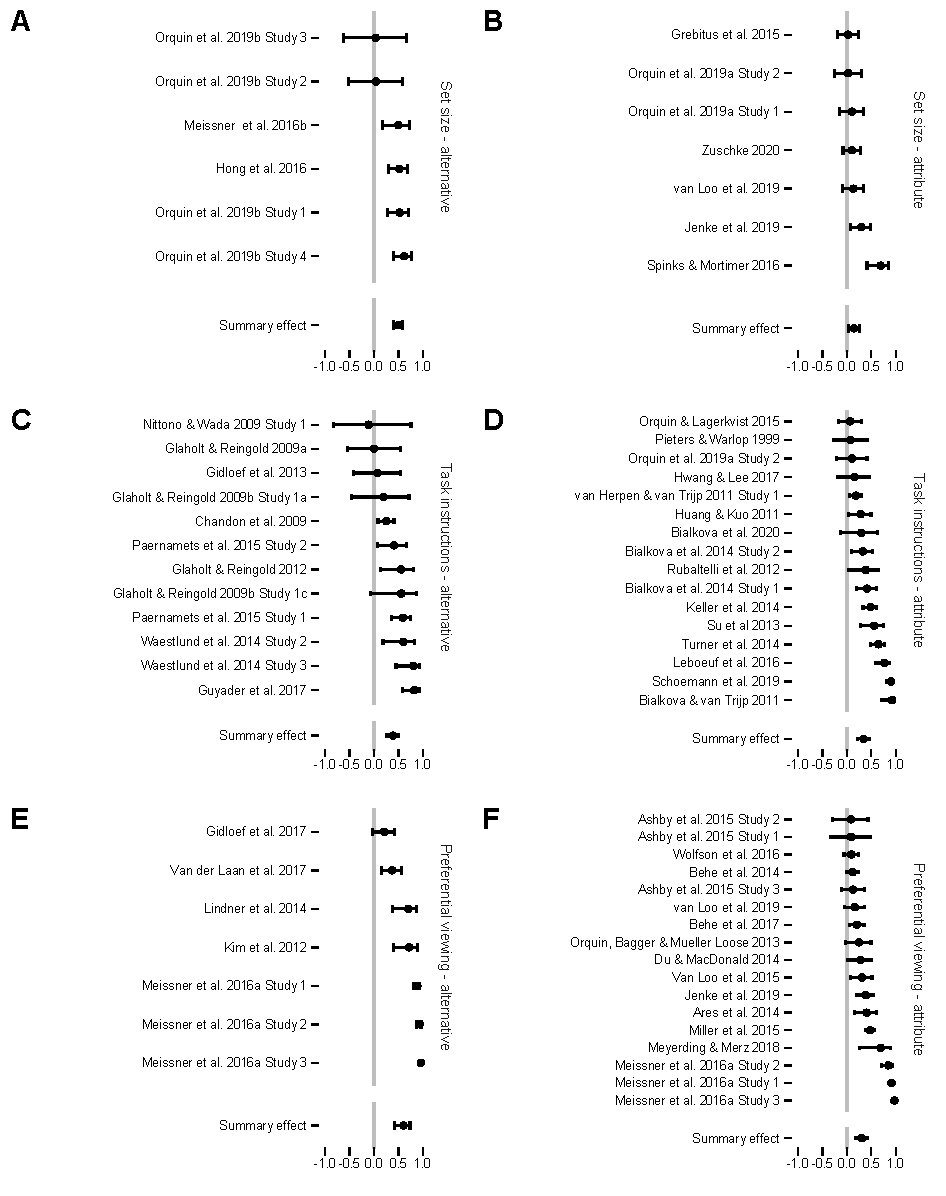
\includegraphics{forest_plots_altatt}
\centering
\singlespace
\caption{Effect sizes of the factors that were decomposed into alternative and attribute parts for moderator analyses. Forest plots show the unattenuated effect size correlations for each study in a group, as well as average effect across the group. Forest plot in (A) shows the effect sizes for set size -- alternative, in (B) for set size -- attribute, in (C) for task instructions -- alternative, in (D) for task instructions -- attribute, in (E) for preferential viewing -- alternative, and in (F) for preferential viewing -- attribute. Error bars represent the 95\% confidence interval around the mean.}
\label{fig:forest_plots_altatt}
\end{figure}
\clearpage


\begin{figure}[!h]
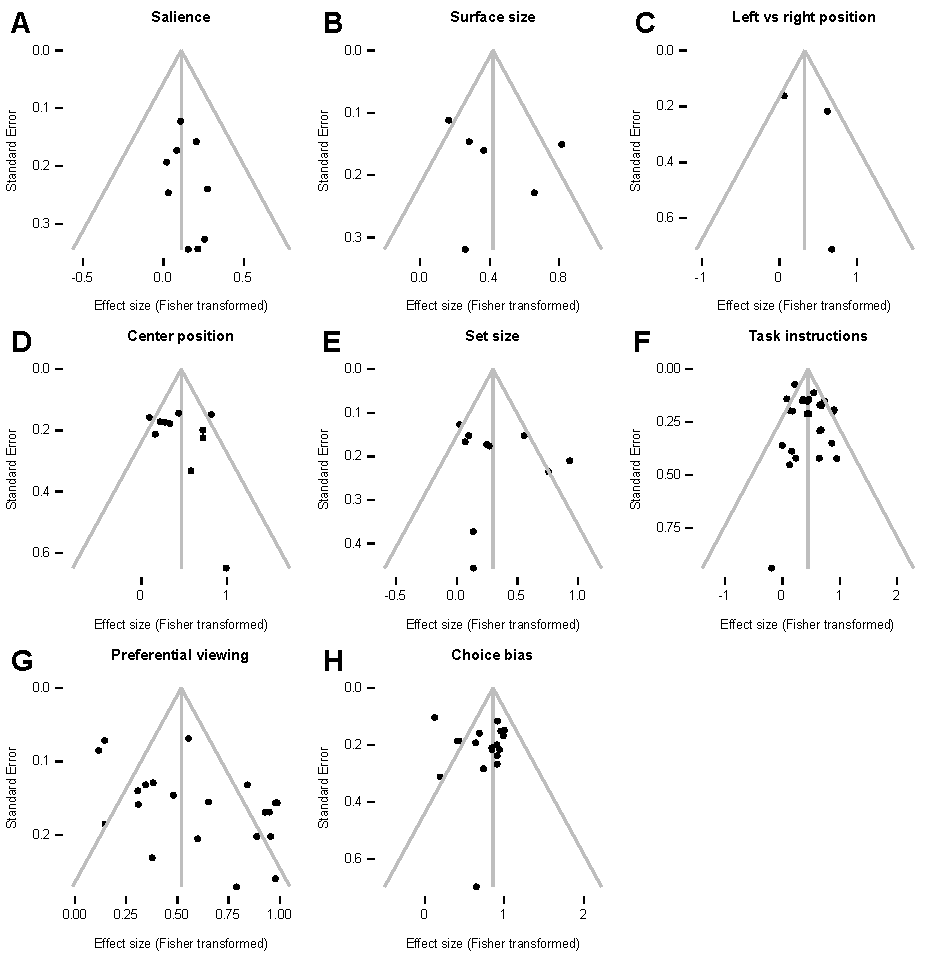
\includegraphics{funnel_plots}
\centering
\caption{Funnel plots for each factor that can be used as a qualitative check of a publication bias. Points are Fisher transformed correlation coefficients against their standard error. Asymmetric distributions of points can indicate the presence of publication bias since smaller studies (those with higher standard errors) have more variable effect sizes and are less likely to be published unless the effect is large. Funnel plot for (A) salience, (B) surface size, (C) left vs right position, (D) central position, (E) set size, (F) task instructions, (G) preferential viewing, and (H) choice-gaze effect.}
\label{fig:funnel_plots}
\end{figure}


\begin{figure}%[H]
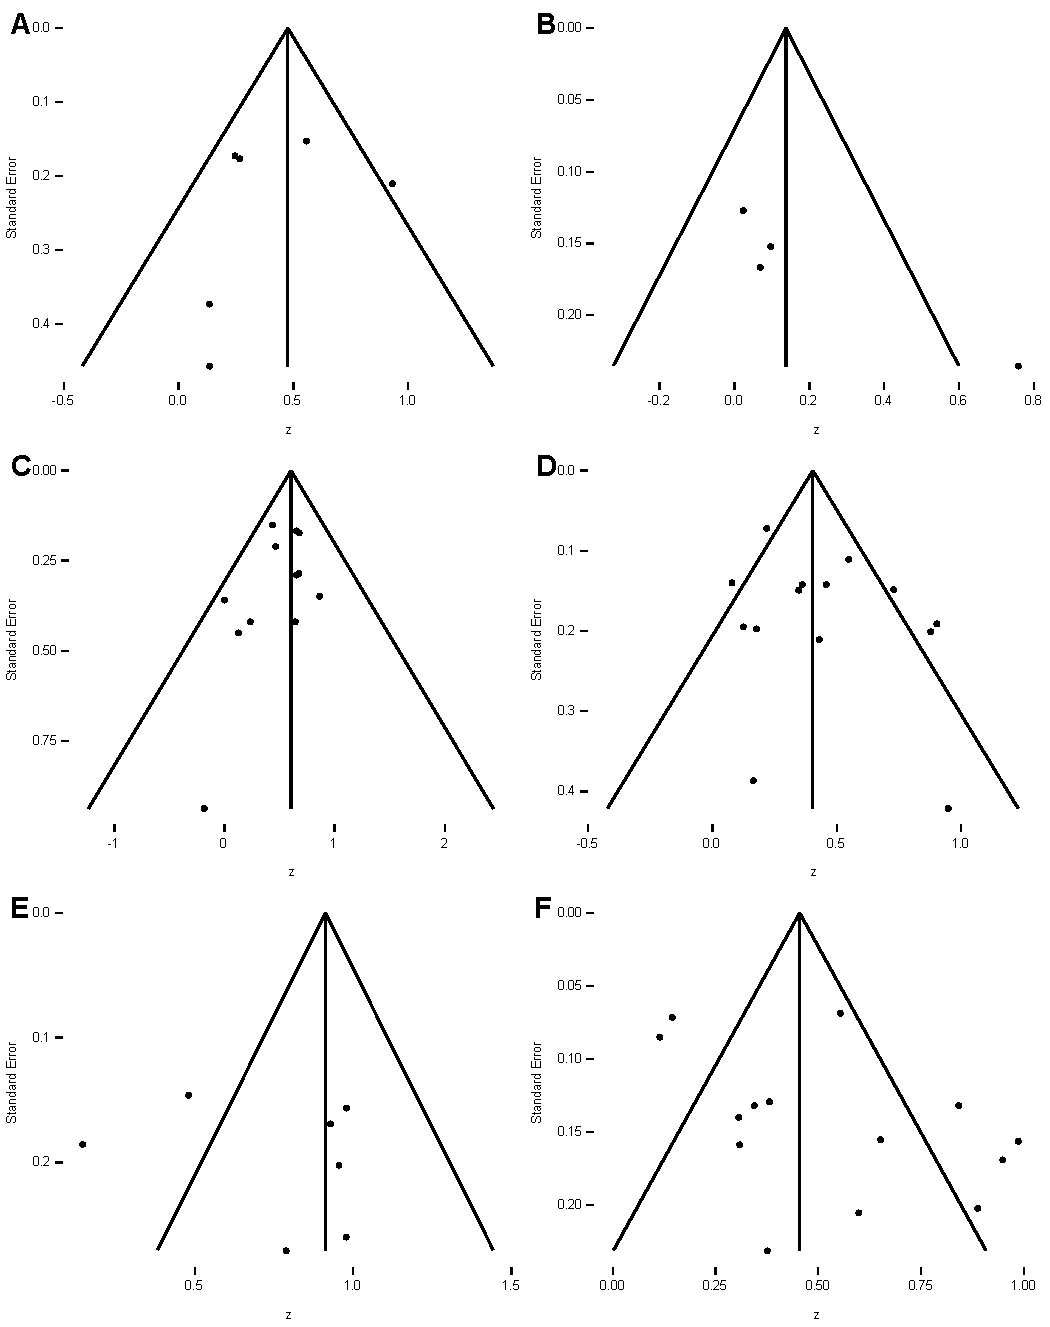
\includegraphics{funnel_plots_altatt}
\centering
\singlespace
\caption{Funnel plots for factors that were decomposed into alternative and attribute parts for moderator analyses. Points are Fisher transformed correlation coefficients against their standard error. Asymmetric distributions of points can indicate the presence of publication bias since smaller studies (those with higher standard errors) have more variable effect sizes and are less likely to be published unless the effect is large. Funnel plot for (A) set size -- alternative, (B) set size -- attribute, (C) task instructions -- alternative, (D) task instructions -- attribute, (E) preferential viewing -- alternative, (F) preferential viewing -- attribute.}
\label{fig:funnel_plots_altatt}
\end{figure}
\clearpage


%\label{tab:overview}
% latex table generated in R 3.5.2 by xtable 1.8-4 package
% Mon Mar 29 16:34:03 2021
\begingroup\footnotesize
\begin{longtable}{p{5cm}lccclll}
\caption{Overview of individual effect sizes: IV = independent variable (LvR = Left vs. right position, Center = Center position, Sal = Salience, Pref = Preferential viewing, Choice = Choice-gaze effect, Task = Task instructions); $N$ = number of participants; $a_a$ = artifact multiplier; $r$ = attenuated effect size correlation expressed in the fixation count metric; Domain = research domain (Pref con = Preferential consumer choice, Pref non-con = Preferential non-consumer choice, Inf con = Inferential consumer choice, Inf non-con = Inferential non-consumer choice, Lotteries = Risky gambles); Alt/Att = Alternative or attribute manipulation.} \\ 
  \hline
Authors & IV & $N$ & $a_a$ & $r$ & Eye-tracker & Domain & Alt/Att \\ 
  \hline
\endhead
\hline
\multicolumn{8}{l}{\footnotesize Continued on next page}
\endfoot
\endlastfoot
 \hline
\cite{ares2014} & Pref & 71 & 0.776 & 0.320 & Tobii T60 & Pref con & Att \\ 
  \cite{ashby2015} & Pref & 27 & 0.821 & 0.069 & Eye gaze tm & Pref con & Att \\ 
  \cite{ashby2015} & Pref & 34 & 0.821 & 0.067 & Eye gaze tm & Pref con & Att \\ 
  \cite{ashby2015} & Pref & 81 & 0.821 & 0.104 & Eye gaze tm & Pref con & Att \\ 
  \cite{atalay2012a} & Center & 63 & 0.776 & 0.187 & Tobii T1750 & Pref con &  \\ 
  \cite{atalay2012a} & Center & 64 & 0.776 & 0.155 & Tobii T1750 & Pref con &  \\ 
  \cite{bagger2016} & Sal & 20 & 0.776 & 0.117 & EyeLink 1000 & Inf con & Att \\ 
  \cite{bagger2016} & Sal & 22 & 0.776 & 0.169 & EyeLink 1000 & Inf con & Att \\ 
  \cite{bagger2016} & Sal & 40 & 0.776 & 0.163 & EyeLink 1000 & Inf con & Att \\ 
  \cite{bagger2016} & Sal & 61 & 0.776 & 0.015 & EyeLink 1000 & Inf con & Att \\ 
  \cite{behe2014} & Pref & 330 & 0.776 & 0.094 & Tobii X1 & Pref con & Att \\ 
  \cite{behe2015} & Choice & 101 & 0.776 & 0.079 & Tobii X1 & Pref con &  \\ 
  \cite{behe2017} & Pref & 214 & 0.776 & 0.159 & Tobii X1 & Pref con & Att \\ 
  \cite{bialkova2011} & Task & 10 & 0.821 & 0.868 & SMI RED & Inf con & Att \\ 
  \cite{bialkova2014a} & Task & 80 & 0.821 & 0.347 & SMI RED & Inf con & Att \\ 
  \cite{bialkova2014a} & Task & 80 & 0.821 & 0.270 & SMI RED & Inf con & Att \\ 
  \cite{bialkova2020} & Task & 30 & 0.776 & 0.232 & SMI unknown & Pref con & Att \\ 
  \cite{bogomolova2020} & Sal & 200 & 0.821 & 0.138 & Tobii T120 & Pref con & Att \\ 
  \cite{brandstatter2014} & Choice & 80 & 0.776 & 0.775 & EyeLink II & Lotteries &  \\ 
  \cite{cavanagh2014} & Choice & 20 & 0.776 & 0.754 & EyeLink 1000 & Lotteries &  \\ 
  \cite{chandon2009a} & LvR & 348 & 0.552 & 0.019 & ISCAN & Pref con &  \\ 
  \cite{chandon2009a} & Center & 348 & 0.552 & 0.347 & ISCAN & Pref con &  \\ 
  \cite{chandon2009a} & Size & 348 & 0.552 & 0.346 & ISCAN & Pref con &  \\ 
  \cite{chandon2009a} & Task & 348 & 0.552 & 0.142 & ISCAN & Pref con & Alt \\ 
  \cite{du2014} & Pref & 72 & 0.821 & 0.228 & Tobii T120 & Pref con & Att \\ 
  \cite{fiedler2012} & Choice & 21 & 0.821 & 0.718 & Eye gaze tm & Lotteries &  \\ 
  \cite{fiedler2012} & Choice & 36 & 0.821 & 0.548 & Eye gaze tm & Lotteries &  \\ 
  \cite{folke2016} & Choice & 28 & 0.776 & 0.750 & EyeLink II & Pref con &  \\ 
  \cite{folke2016} & Choice & 24 & 0.776 & 0.808 & EyeLink 1000 & Pref con &  \\ 
  \cite{gidloef2017a} & Choice & 260 & 0.458 & 0.207 & SMI Glasses & Pref con &  \\ 
  \cite{gidloef2017a} & Center & 260 & 0.458 & 0.523 & SMI Glasses & Pref con &  \\ 
  \cite{gidloef2017a} & Pref & 260 & 0.458 & 0.095 & SMI Glasses & Pref con & Alt \\ 
  \cite{gidloef2017a} & Sal & 260 & 0.458 & 0.019 & SMI Glasses & Pref con &  \\ 
  \cite{gidloef2017a} & Size & 260 & 0.458 & 0.464 & SMI Glasses & Pref con &  \\ 
  \cite{gidlof2013} & Task & 40 & 0.552 & 0.040 & SMI iview HED & Pref con & Alt \\ 
  \cite{glaholt2009a} & Task & 16 & 0.776 & 0.000 & EyeLink 1000 & Inf non-con & Alt \\ 
  \cite{glaholt2009b} & Choice & 12 & 0.776 & 0.096 & EyeLink 1000 & Inf non-con &  \\ 
  \cite{glaholt2009b} & Choice & 12 & 0.776 & 0.153 & EyeLink 1000 & Pref non-con &  \\ 
  \cite{glaholt2009b} & Task & 12 & 0.776 & 0.153 & EyeLink 1000 & Inf non-con & Alt \\ 
  \cite{glaholt2009b} & Task & 12 & 0.776 & 0.455 & EyeLink 1000 & Inf non-con & Alt \\ 
  \cite{glaholt2009c} & Choice & 16 & 0.776 & 0.755 & EyeLink 1000 & Inf non-con &  \\ 
  \cite{glaholt2010} & LvR & 48 & 0.776 & 0.545 & EyeLink 1000 & Inf non-con &  \\ 
  \cite{glaholt2010} & Center & 48 & 0.776 & 0.645 & EyeLink 1000 & Inf non-con &  \\ 
  \cite{glaholt2012} & Choice & 24 & 0.776 & 0.646 & EyeLink 1000 & Inf non-con &  \\ 
  \cite{glaholt2012} & Task & 24 & 0.776 & 0.451 & EyeLink 1000 & Inf non-con & Alt \\ 
  \cite{graham2016} & Size & 155 & 0.776 & 0.106 & EyeLink 1000 & Pref con &  \\ 
  \cite{grebitus2015} & Set size & 130 & 0.776 & 0.019 & Tobii T60 & Pref con & Att \\ 
  \cite{guyader2017} & Task & 66 & 0.458 & 0.487 & SMI Glasses & Inf con & Alt \\ 
  \cite{hong2016a} & Set size & 75 & 0.821 & 0.440 & Tobii T120 & Pref con & Alt \\ 
  \cite{huang2011} & Task & 88 & 0.776 & 0.221 & EyeLink II & Pref non-con & Att \\ 
  \cite{hwang2017} & Task & 42 & 0.821 & 0.126 & Tobii X2 & Inf con & Att \\ 
  \cite{jenke2019} & Pref & 122 & 0.776 & 0.308 & Tobii T60 & Inf non-con & Att \\ 
  \cite{jenke2019} & Set size & 122 & 0.776 & 0.230 & Tobii T60 & Inf non-con & Att \\ 
  \cite{keller2014} & Task & 159 & 0.776 & 0.388 & SMI iview & Inf non-con & Att \\ 
  \cite{kim2012a} & Pref & 24 & 0.776 & 0.610 & EyeLink II & Lotteries & Alt \\ 
  \cite{krajbich2010a} & Choice & 39 & 0.776 & 0.926 & Tobii T2150 & Pref con &  \\ 
  \cite{kreplin2014a} & LvR & 19 & 0.552 & 0.270 & ASL6000 & Pref non-con &  \\ 
  \cite{kreplin2014a} & Center & 19 & 0.552 & 0.730 & ASL6000 & Pref non-con &  \\ 
  \cite{kwak2018} & LvR & 63 & 0.776 & 0.453 & Tobii T60 & Lotteries & Alt \\ 
  \cite{leboeuf2016} & Task & 54 & 0.776 & 0.652 & EyeLink 1000 & Inf con & Att \\ 
  \cite{lindner2014} & Choice & 30 & 0.776 & 0.453 & SMI iview & Inf non-con &  \\ 
  \cite{lindner2014} & Pref & 26 & 0.776 & 0.588 & SMI iview & Inf non-con & Alt \\ 
  \cite{lohse1997a} & Sal & 32 & 0.679 & 0.077 & Eye gaze 97 & Pref con &  \\ 
  \cite{lohse1997a} & Size & 32 & 0.679 & 0.174 & Eye gaze 97 & Pref con &  \\ 
  \cite{meissner2016a} & Center & 60 & 0.776 & 0.230 & EyeLink II & Pref con &  \\ 
  \cite{meissner2016a} & Pref & 60 & 0.776 & 0.798 & EyeLink II & Pref con & Alt \\ 
  \cite{meissner2016a} & Pref & 60 & 0.776 & 0.836 & EyeLink II & Pref con & Att \\ 
  \cite{meissner2016a} & Center & 35 & 0.821 & 0.120 & Tobii T120 & Pref con &  \\ 
  \cite{meissner2016a} & Pref & 35 & 0.821 & 0.775 & Tobii T120 & Pref con & Att \\ 
  \cite{meissner2016a} & Pref & 35 & 0.821 & 0.881 & Tobii T120 & Pref con & Alt \\ 
  \cite{meissner2016a} & Pref & 70 & 0.776 & 0.906 & Tobii T2150 & Pref con & Alt \\ 
  \cite{meissner2016a} & Pref & 70 & 0.776 & 0.930 & Tobii T2150 & Pref con & Att \\ 
  \cite{meissner2016a} & Center & 70 & 0.692 & 0.220 & Unknown & Pref con &  \\ 
  \cite{meissner2016b} & Set size & 40 & 0.821 & 0.420 & Tobii T120 & Pref con & Alt \\ 
  \cite{meyerding2018} & Pref & 73 & 0.364 & 0.301 & Tobii glasses 2 & Pref con & Att \\ 
  \cite{miller2015} & Pref & 358 & 0.776 & 0.382 & EyeLink 1000 & Pref con & Att \\ 
  \cite{mitsuda2014} & Choice & 48 & 0.776 & 0.842 & EyeLink II & Inf non-con &  \\ 
  \cite{neuhofer2020} & Size & 164 & 0.821 & 0.238 & Tobii X2 & Pref con & Att \\ 
  \cite{nittono2009} & Choice & 10 & 0.552 & 0.248 & Nihon-Kohden & Inf non-con &  \\ 
  \cite{nittono2009} & Task & 10 & 0.552 & -0.062 & Nihon-Kohden & Inf non-con & Alt \\ 
  \cite{orquin2013} & Pref & 68 & 0.776 & 0.195 & Tobii T2150 & Pref con & Att \\ 
  \cite{orquin2015a} & Sal & 150 & 0.776 & 0.067 & Tobii T60 & Pref con & Att \\ 
  \cite{orquin2015a} & Task & 100 & 0.776 & 0.052 & Tobii T60 & Pref con & Att \\ 
  \cite{orquin2019a} & Center & 91 & 0.776 & 0.267 & Tobii T2150 & Pref con & Att \\ 
  \cite{orquin2019a} & Sal & 91 & 0.776 & 0.088 & Tobii T2150 & Pref con & Att \\ 
  \cite{orquin2019a} & Set size & 91 & 0.776 & 0.078 & Tobii T2150 & Pref con & Att \\ 
  \cite{orquin2019a} & Size & 91 & 0.776 & 0.222 & Tobii T2150 & Pref con & Att \\ 
  \cite{orquin2019a} & Center & 76 & 0.776 & 0.068 & EyeLink 1000 & Inf con & Att \\ 
  \cite{orquin2019a} & Sal & 76 & 0.776 & 0.048 & EyeLink 1000 & Inf con & Att \\ 
  \cite{orquin2019a} & Set size & 76 & 0.776 & 0.020 & EyeLink 1000 & Inf con & Att \\ 
  \cite{orquin2019a} & Size & 76 & 0.776 & 0.230 & EyeLink 1000 & Inf con & Att \\ 
  \cite{orquin2019a} & Task & 52 & 0.776 & 0.083 & EyeLink 1000 & Inf con & Att \\ 
  \cite{orquin2020osfb} & Set size & 71 & 0.776 & 0.423 & Tobii T60 & Pref con & Alt \\ 
  \cite{orquin2020osfb} & Set size & 16 & 0.776 & 0.033 & Tobii T60 & Pref con & Alt \\ 
  \cite{orquin2020osfb} & Set size & 11 & 0.776 & 0.027 & Tobii T60 & Pref con & Alt \\ 
  \cite{orquin2020osfb} & Set size & 68 & 0.776 & 0.508 & Tobii T60 & Pref con & Alt \\ 
  \cite{paernamets2015a} & Task & 58 & 0.821 & 0.504 & SMI RED & Pref non-con & Alt \\ 
  \cite{paernamets2015a} & Task & 37 & 0.821 & 0.342 & SMI RED & Pref non-con & Alt \\ 
  \cite{peschel2019} & Sal & 127 & 0.776 & 0.004 & Tobii T60 & Pref con & Att \\ 
  \cite{peschel2019} & Size & 127 & 0.776 & 0.098 & Tobii T60 & Pref con & Att \\ 
  \cite{pieters1999} & Task & 54 & 0.692 & 0.051 & Unknown & Pref con & Att \\ 
  \cite{robertson2020} & LvR & 74 & 0.776 & 0.130 & EyeLink 1000* & Pref con & Att \\ 
  \cite{rubaltelli2012} & Task & 37 & 0.821 & 0.324 & Eye gaze tm & Lotteries & Att \\ 
  \cite{schoemann2019} & Task & 40 & 0.852 & 0.855 & EyeLink 1000** & Lotteries & Att \\ 
  \cite{schotter2010a} & Choice & 32 & 0.776 & 0.262 & EyeLink II & Inf non-con &  \\ 
  \cite{schotter2010a} & Choice & 32 & 0.776 & 0.290 & EyeLink II & Pref non-con &  \\ 
  \cite{schotter2012a} & Choice & 32 & 0.776 & 0.292 & EyeLink 1000 & Inf non-con &  \\ 
  \cite{spinks2016a} & Set size & 32 & 0.821 & 0.602 & Tobii T120 & Inf non-con & Att \\ 
  \cite{su2013} & Task & 49 & 0.776 & 0.454 & EyeLink II & Lotteries & Att \\ 
  \cite{turner2014} & Task & 89 & 0.776 & 0.534 & Tobii D10 & Pref con & Att \\ 
  \cite{vanderlaan2015} & Choice & 22 & 0.687 & 0.451 & Easygaze & Inf con &  \\ 
  \cite{vanderlaan2017} & Pref & 125 & 0.687 & 0.263 & Easygaze & Pref con & Alt \\ 
  \cite{vanherpen2011} & Task & 309 & 0.821 & 0.150 & SMI RED & Pref con & Att \\ 
  \cite{vanloo2015} & Pref & 81 & 0.821 & 0.257 & SMI RED & Pref con & Att \\ 
  \cite{vanloo2019} & Set size & 103 & 0.821 & 0.110 & Tobii X2 & Pref con & Att \\ 
  \cite{vanloo2019} & Pref & 103 & 0.821 & 0.132 & Tobii X2 & Pref con & Att \\ 
  \cite{wastlund2015} & Task & 98 & 0.364 & 0.247 & Tobii Glasses 1 & Inf con & Alt \\ 
  \cite{wastlund2015} & Task & 66 & 0.364 & 0.381 & Tobii Glasses 1 & Inf con & Alt \\ 
  \cite{wolfson2017} & Pref & 234 & 0.776 & 0.071 & EyeLink 1000 & Pref con & Att \\ 
  \cite{zuschke2020} & Sal & 172 & 0.776 & 0.262 & Tobii X60 & Pref con & Att \\ 
  \cite{zuschke2020} & Size & 172 & 0.776 & 0.303 & Tobii X60 & Pref con & Att \\ 
  \cite{zuschke2020} & Set size & 172 & 0.776 & 0.080 & Tobii X60 & Pref con & Att \\ 
  \hline
\label{tab:overviewtable}
\end{longtable}
\endgroup


